\subsection{Random Forest}

Random forest is an algorithm developed from decision tree. Trees that are grown very deep tend to learn highly irregular patterns: they overfit their training sets. Random forest is a way of averaging multiple deep decision trees, trained on different parts of the same training set, with the goal of reducing the variance. This comes at the expense of a small increase in the bias and some loss of interpretability, but generally greatly boosts the performance in the final model.

The major advantage of random forest is that it is robust against colinearity, and we can rank the importance of variable based on out-of-bag error\cite{breiman2001random}. As it is easy to carry out and require no data assumption, we decided to first run it to get a better idea about which variable is more vital in weather forecast. 

\begin{figure}[h]
\centering
\begin{minipage}[t]{0.48\textwidth}
\centering
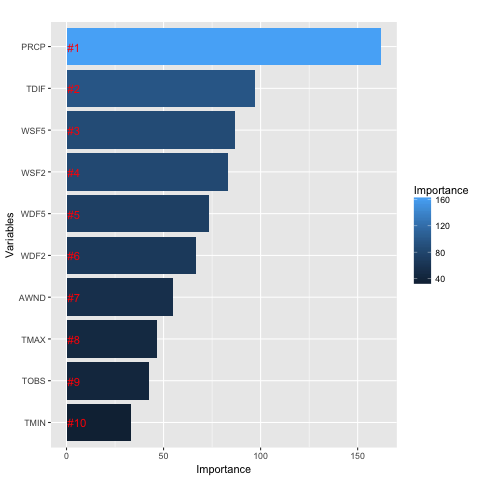
\includegraphics[width = .99\textwidth]{vimp.png}
\caption{Importance of Attributes}
\label{vimp}
\end{minipage}
\begin{minipage}[t]{0.48\textwidth}
\centering
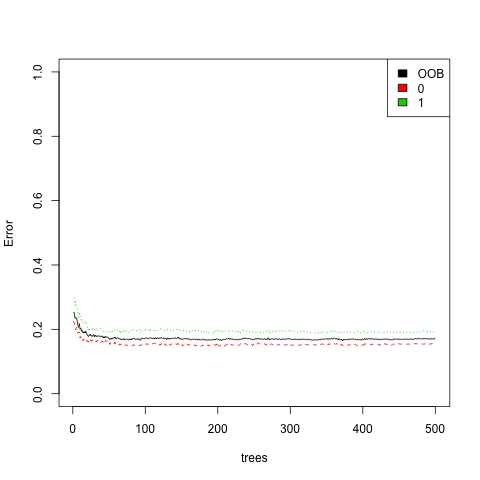
\includegraphics[width = .99\textwidth]{errf.png}
\caption{Error Rate of Random Forest on Training Data}
\label{errf}
\end{minipage}
\end{figure}

As shown in Figure \ref{vimp}, the PRCP is the most important variable. This is intuitively correct as it is the most relative variable. Also we can see our feature engineering plays an important role. The TDIF (temperature difference) and other variables about wind are ranking from \engordnumber{2} to \engordnumber{6}. This give us a sense of what variable should be used in the $k$-NN, since $k$-NN prefers a lower dimension input data.

In Figure \ref{errf}, the error rate become stable when tree number is greater than 100. As the green line is the error rate of predicting days with precipitation and the red line is for days without. The model has a better ability in predicting days without precipitation. This can be numerically confirmed from the confusion matrix in Table \ref{tblrf}. The type \uppercase\expandafter{\romannumeral1} error is higher than type \uppercase\expandafter{\romannumeral2} error, which means the model makes more mistake in predicting days with precipitation. The overall test errors are shown in Table \ref{tblrf}.

Although random forest has many advantages, it still can't deal with the situation when data are not linear separable. So in that case we should try kernel SVM for the next step.

\begin{table}[h]
\setlength{\belowcaptionskip}{5pt}
\caption{Confusion Matrix and Error Rates of Random Forest}
\label{tblrf}
\centering
\renewcommand\arraystretch{1.5}
\begin{tabular}{rrrrr}
\hline
\hline
 & & \multicolumn{2}{c}{True Condition} & \\
\hline
 & & Non-Precipitation & Precipitation & \\
\cline{1-4}
\multirow{2}{*}{Prediction} & {Non-Precipitation} & 339 & 51 & \\
\cline{2-4}
&Precipitation&52&217&\\
\hline
&Error Rate & 0.1329 & 0.1902 & 0.1562\\
\cline{2-5}
& & Type \uppercase\expandafter{\romannumeral1} & Type \uppercase\expandafter{\romannumeral2} & Overall\\
\hline
\end{tabular}
\end{table}